%%%%%%%%%%%%%%%%%%%%%%%%%%%%%%%%%%%%%
%                                   %
% Compile with XeLaTeX and biber    %
%                                   %
% Questions or comments:            %
%                                   %
% joshua dot mcneill at uga dot edu %
%                                   %
%%%%%%%%%%%%%%%%%%%%%%%%%%%%%%%%%%%%%

\documentclass{beamer}
  % Read in standard preamble (cosmetic stuff)
  %%%%%%%%%%%%%%%%%%%%%%%%%%%%%%%%%%%%%%%%%%%%%%%%%%%%%%%%%%%%%%%%
% This is a standard preamble used in for all slide documents. %
% It basically contains cosmetic settings.                     %
%                                                              %
% Joshua McNeill                                               %
% joshua dot mcneill at uga dot edu                            %
%%%%%%%%%%%%%%%%%%%%%%%%%%%%%%%%%%%%%%%%%%%%%%%%%%%%%%%%%%%%%%%%

% Beamer settings
% \usetheme{Berkeley}
\usetheme{CambridgeUS}
% \usecolortheme{dove}
% \usecolortheme{rose}
\usecolortheme{seagull}
\usefonttheme{professionalfonts}
\usefonttheme{serif}
\setbeamertemplate{bibliography item}{}

% Packages and settings
\usepackage{fontspec}
  \setmainfont{Charis SIL}
\usepackage{hyperref}
  \hypersetup{colorlinks=true,
              allcolors=blue}
\usepackage{graphicx}
  \graphicspath{{../../figures/}}
\usepackage[normalem]{ulem}
\usepackage{enumerate}

% Document information
\author{M. McNeill}
\title[FREN2001]{Français 2001}
\institute{\url{joshua.mcneill@uga.edu}}
\date{}

%% Custom commands
% Lexical items
\newcommand{\lexi}[1]{\textit{#1}}
% Gloss
\newcommand{\gloss}[1]{`#1'}
\newcommand{\tinygloss}[1]{{\tiny`#1'}}
% Orthographic representations
\newcommand{\orth}[1]{$\langle$#1$\rangle$}
% Utterances (pragmatics)
\newcommand{\uttr}[1]{`#1'}
% Sentences (pragmatics)
\newcommand{\sent}[1]{\textit{#1}}
% Base dir for definitions
\newcommand{\defs}{../definitions}


  % Packages and settings

  % Document information
  \subtitle[Présentons-nous]{Présentons-nous}

  %% Custom commands
  % Subsection/frame titles

\begin{document}
  % Read in the standard intro slides (title page and table of contents)
  \begin{frame}
    \titlepage
    \tiny{Office: % Basically a variable for office hours location
Gilbert 121\\
          Office hours: % Basically a variable for office hours
 lundi, mercredi, vendredi 10:10--11:10
}
  \end{frame}

  \begin{frame}{Qui est-ce?}
    \gloss{Say who that is and confirm with a \lexi{pronom disjoint}.}
    \centering
    
\includegraphics[scale=0.22]{hulk_et_she-hulk.jpg}

    \uncover<2->{
      Ce sont \alert<3->{Hulk et She-Hulk}.
    }

    \uncover<3->{
      Ce sont \alert{eux}.
    }
  \end{frame}

  \begin{frame}{Qui est-ce?}
    \centering
    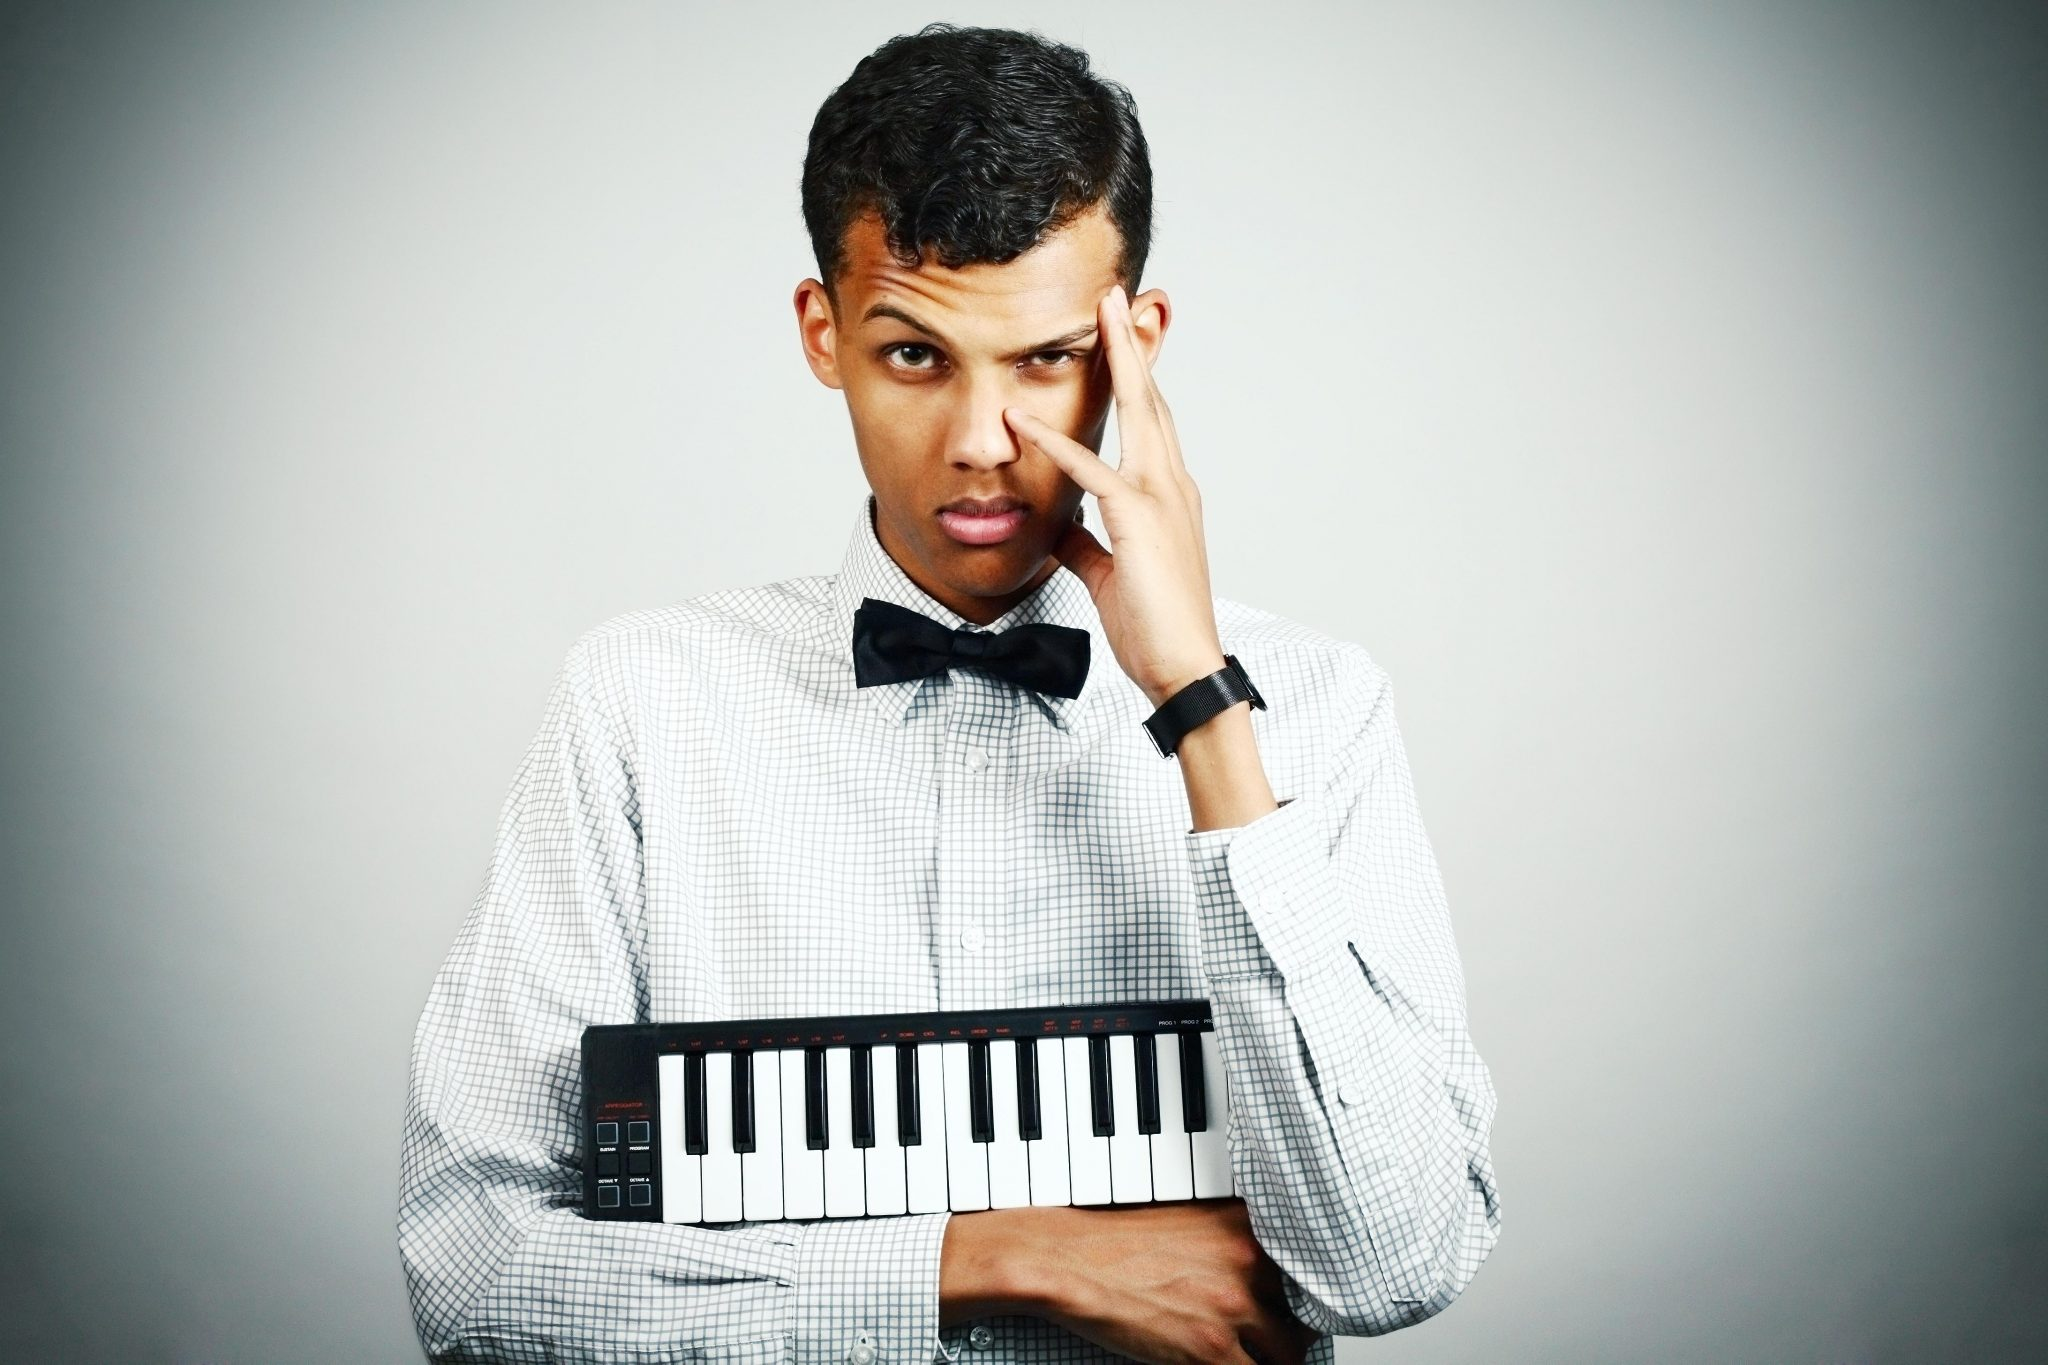
\includegraphics[scale=0.15]{stromae.jpg}

    \uncover<2->{
      C'est \alert<3->{Stromae}.
    }

    \uncover<3->{
      C'est \alert{lui}.
    }
  \end{frame}

  \begin{frame}{Toi ou vous?}
    \gloss{Find a partner, and imagine that they are the person on their card.
    Introduce yourself, ask them how they are doing, and tell them how you are doing.
    For example:}

    <E1 $\to$ teacher, E2 $\to$ student>
    \begin{itemize}
      \item[E1:] Bonjour, je m'appelle Monsieur McNeill. Comment tu t'appelles?
      \item[E2:] Bonjour, je m'appelle ...
      \item[E1:] Comment ça va?
      \item[E2:] Je suis fatigué, et vous?
      \item[E1:] Je vais bien.
    \end{itemize}
  \end{frame}
\end{document}
